\chapter{Implementacja projektu - monolit}
\label{roz4}
W tym rozdziale pokrótce zostanie opisana implementacja projektu monolitycznego. Został on podzielony według wcześniejszych założeń architektonicznych~i obejmować będzie procedury potrzebne do napisania aplikacji serwerowej~w \textit{frameworku} \textit{Flask} i szablonów \textit{HTML} przy wykorzystaniu \textit{Vue.js} i innych technologii webowych takich jak \textit{Javascript}, \textit{HTML} i \textit{CSS}.
%=================================================================================================
\section{Backend}
Sekcja ta odpowiada za opisanie implementacji od strony serwera, której zadaniem jest przyjmowanie zapytań, a następnie zwracanie odpowiadających im szablonów \textit{HTML}. Za ich pomocą użytkownik może podejmować interakcję~z stroną~i używając wygenerowanych formularzy tworzyć kolejne żądania, na które program musi odpowiednio zareagować.

Pierwszym wykonanym krokiem było stworzenie nowego projektu~o nazwie \textit{mono}. Następnie wewnątrz niego utworzono katalog~o tej samej nazwie~i~w jego środku dodano nowy folder \textit{\_\_init\_\_.py}. Odpowiada on za import wszystkich innych modułów, a także stworzenie instancji dla głównej klasy~z biblioteki \textit{Flask}\cite{flask}. Ważne jest, zwrócenie uwagi na to, że silnik wykorzystany do generowania szablonów \textit{Jinja2}, ma takie same elementy składni jak \textit{Vue.js} i niemożliwe ich jednoczesne wykorzystanie, chyba, że zmienione zostaną ustawienie jednego~z nich\cite{vuejs, flask}. W tym celu zaimplementowano klasę \textit{VueFlask}, która dziedziczy po \textit{Flask}, a następnie przypisano~w niej skopiowany słownik\footnote{Struktura danych składająca się~z klucza~i jego wartości\cite{python}, dobrze nadaje się do zapisywania~w niej różnego rodzaju ustawień.} z ustawieniami \textit{Jinja}. Korzystając~z metody \textit{update}\cite{python} nadpisano klucze odpowiadające za deklarowanie zmiennych wewnątrz plików \textit{HTML}. Kod klasy prezentuje się następująco:

\newpage
\begin{lstlisting}[language=Python, caption={Zmiana opcji silnika \textit{Jinja2} poprzez nadpisanie klasy \textit{Flask}.}]
from flask import Flask

class VueFlask(Flask):
    jinja_options = Flask.jinja_options.copy()
    jinja_options.update(dict(
        variable_start_string='%%',
        variable_end_string='%%',
    ))
app = VueFlask(__name__)
\end{lstlisting}

Klasa \textit{VueFlask} przyjmuje argument \textit{\_\_name\_\_}, jest to zmienna globalna zawierająca nazwę obecnego modułu~i przekazanie jej jest wymagana przez dokumentacje \textit{Flaska}\cite{flask}.

W podobny sposób potrzebne jest stworzenie instancji dla biblioteki \textit{Flask SQLAlchemy}, tak samo wymagane jest zaimportowanie klasy~i przypisanie jej do zmiennej \textit{db}, podając jako argument wcześniej utworzony obiekt \textit{app}. Daje to możliwość zaprojektowanie modeli dla użytkowników~i zadań.

\subsection{Modele}
Wszystkie modele będą umiejscowione~w pliku \textit{models.py} i zaprojektowane jako klasy dziedziczące po obiekcie \textit{db.Model}\cite{flasksql}. Jako pierwszy został stworzony model użytkownika posiadający pola, \textit{id}, unikalny identyfikator dla wszystkich użytkowników opisany wyłącznie przy pomocy liczb całkowitych. \textit{Username}, kolumnę~w bazie danych, zapisaną za pomocą ciągu znaków, mających długość \textit{32} liter. \textit{Email}, podobnie jak jego poprzednik, to również ciąg znaków długości \textit{64} liter~i \textit{password}, mające maksymalna długość \textit{128} znaków. Zgodnie~z ustaleniami~z rozdziału \ref{sec:problemy}, hasła nie będą~w bazie danych zapisane zwykłym tekstem, tylko szyfrowane. W związku~z tym klasa posiada jeszcze dwie metody odpowiedzialne za ich utajnienie~i sprawdzanie zgodności~z haszem\cite{Ziade:2018}. 
\begin{lstlisting}[language=Python, caption={Klasa odpowiedzialna za model użytkownika.}]
from werkzeug.security import generate_password_hash, check_password_hash
from datetime import datetime
from mono import db


class User(db.Model):
    id = db.Column(db.Integer, primary_key=True)
    username = db.Column(db.String(32), index=True, unique=True)
    email = db.Column(db.String(64), index=True, unique=True)
    password_hash = db.Column(db.String(128))

    def set_password(self, password):
        self.password_hash = generate_password_hash(password)

    def check_password(self, password):
        return check_password_hash(self.password_hash, password)
\end{lstlisting}

Kolejnym modelem jest ten odpowiedzialny za definiowanie zadań. Posiada on także pole \textit{id} będące unikatową liczbą identyfikującą każde~z nich. Dzięki polu \textit{is\_done}, które jest typu \textit{prawda$/$fałsz}\footnote{Z angielskiego \textit{Boolean}, trzymające informację binarną~o stanie logicznym\cite{flasksql}.} użytkownik może oznaczyć zdanie jako skończone lub nie. Każdy zapisany~w bazie danych cel będzie składał się~z tytułu (\textit{header}) i jego opisu (\textit{body}). Obie własności są kolumnami typu \textit{string} zawierających ich~w kolejności \textit{64} i \textit{256}. Ostatnim polem~w tym modelu jest stempel czasu (ang. \textit{time stamp}) trzymającym dane~o dacie~i dokładnym czasie (zgodnym~z formatem \textit{utc}\cite{python} zawierającym godziny, minuty, sekundy~i milisekundy), jego wartość jest natychmiastowo przypisywana, przy utworzeniu zadania, na podstawie aktualnych informacji~z systemu\cite{python}.

\begin{lstlisting}[language=Python, caption={Klasa odpowiedzialna za model zadania.}]
from datetime import datetime # wymagany import umieszczony na poczatku pliku


class Task(db.Model):
    id = db.Column(db.Integer, primary_key=True)
    is_done = db.Column(db.Boolean)
    header = db.Column(db.String(68))
    body = db.Column(db.String(256))
    timestamp = db.Column(db.DateTime, index=True, default=datetime.utcnow)
\end{lstlisting}
%============================================= ====================================================

Brak jeszcze informacji~o korelacji między użytkownikiem, a zadaniem. Zgodnie~z schematem opisanym~w rozdziale \ref{sec:bazadanych}. Jedna osoba korzystająca~z aplikacji może mieć wiele stworzonych przez siebie celi, natomiast jeden taki cel może mieć tylko jednego autora. Dlatego wewnątrz klasy \textit{User} należy dodać pole \textit{task}, tworząc powiązanie \textit{db.relationship}, odpowiadające relacji \textit{one-to-many}\cite{flasksql} z referencją wsteczną do zadania, o nazwie \textit{author}. Oznacza to, że będzie można odnieść się od strony użytkownika do utworzonych przez niego zadań dzięki temu, że będą one miały~w bazie danych tabelę \textit{author} posiadającą informacje umożliwiając jego identyfikację.

Natomiast relacja pomiędzy zadaniem~i jego właścicielem opisana jest jako \textit{one-to-many}, nazywana również \textit{Foreign Key}\cite{Ziade:2018, flasksql} i do jej utworzenia należy po prostu zapisać~w modelu \textit{user\_id} będącą kolumną numeryczna, która jako drugi argument przyjmuje \textit{db.ForeignKey('user.id')} z odniesieniem właśnie do identyfikatora użytkownika.

Samo utworzenie modeli~w języku \textit{Python} nie wystarczy, aby baza danych przyjęła wymaganą strukturę. Najpierw trzeba skonfigurować połączenie~z nią. W folderze głównym projektu utworzono plik \textit{.env} przechowujący wszystkie dane na temat środowiska, są~w nim opisane informacje~o bazie danych, tym, czy aplikacja działa~w trybie produkcyjnym, czy powinna wyświetlać informacje~o błędach (tryb \textit{debug})\cite{flask}. Są one wczytywane przez plik \textit{config.py} i mapowane na klasy dotyczące danego środowiska konfiguracyjnego\footnote{Istnieją różne środowiska, w których aplikacja może zostać uruchomiona takie jak testowe, produkcyjne lub deweloperskie.}, a na końcu za pomocą funkcji~z biblioteki \textit{Flask} o nazwie \textit{config.from\_object}\cite{flask}, wczytywane do opisanej wcześniej instancji biblioteki, zmiennej \textit{app}.
\newpage
\begin{lstlisting}[language=Python, caption={Klasa odpowiedzialna za wczytywanie i zapisanie konfiguracji międzyinnymi bazy danych.}]
POSTGRES = {
    'user': os.environ.get('DB_USER'),
    'pw': os.environ.get('DB_PASS'),
    'db': os.environ.get('DB_NAME'),
    'host': os.environ.get('DB_ADDRESS'),
    'port': os.environ.get('DB_PORT'),
}


class Config:
    DEBUG = False
    SECRET_KEY = os.environ.get('SECRET_KEY')
    SQLALCHEMY_TRACK_MODIFICATIONS = False
    SQLALCHEMY_DATABASE_URI = 'postgresql://%(user)s:\
        %(pw)s@%(host)s:%(port)s/%(db)s' % POSTGRES


class ConfigDevelopment(Config):
    DEBUG = True
\end{lstlisting}

Aplikacja do poprawnego działania potrzebuje takich informacji jak nazwa użytkownika, login administratora bazy danych, jego hasło, nazwa bazy~i adres, na którym znajduje się włączona usługa. Zmienne mające~w nazwie \textit{SQLALCHEMY} są wymagane do uzupełnienia przez bibliotekę \textit{Flask SQLAlchemy} i potrzebne do jej działania. Proces konfiguracji już samej bazy danych \textit{Postresql} zostany dokładniej opisany~w rozdziale~o konteneryzacji aplikacji (rozdz. \ref{roz6}).

%TODO: Dodać ref do konfiguracji aplikacji

Proces tworzenie struktur lub aktualizowania bazy danych~o wcześniej zdefiniowane modele, to migracje. Powinno je się wykonać po każdej zmianie~w kodzie \textit{models.py} i uruchomieniu nowo stworzonej bazy danych\cite{django}. Do ich obsługi~w systemie \textit{Flask} istnieje narzędzie~o nazwie \textit{Alemibic}\footnote{Link do dokumentacji \textit{Alembica}: \url{https://alembic.sqlalchemy.org/en/latest/}.} i jest ono częścią biblioteki \textit{Flask Migration}\footnote{Link do dokumentacji pakietu \textit{Flask Migration}: \url{https://flask-migrate.readthedocs.io/en/latest/}.}.

Uruchomienie migracji nie będzie wiązało się~z włączeniem aplikacji\cite{Grinberg:2017}, ale będą one tworzone na żądanie osoby nią operującą, dlatego potrzebne będzie dodanie do zbioru komend \textit{Flaska}\cite{flask} nowych, odpowiedzialnych za włączenie \textit{Alembica}. Do tego potrzebna będzie jeszcze jedna biblioteka~o nazwie \textit{Flask Script}\footnote{Link do dokumentacji biblioteki \textit{Flask Script}: \url{https://flask-script.readthedocs.io/en/latest/}.}, a następnie dopisanie do pliku \textit{mono$/$\_\_init\_\_.py} następujący fragmentów kodu:
 
\begin{lstlisting}[language=Python, caption={Dodanie migracji do skryptu \textit{Flaska} w pliku \textit{mono$/$\_\_init\_\_.py}.}]
migrate = Migrate(app, db)
manager = Manager(app)

manager.add_command('db', MigrateCommand) 
\end{lstlisting}

Wówczas możliwe będzie uruchomienie~w konsoli polecenia \verb|flask db init| (w głównym katalogu projektu) do inicjalizowania połączenia modeli~z bazią danych, a następnie \verb|flask db migrate| do utworzenia plików migracyjnych. W katalogu powinien pojawić się nowy folder~o nazwie \textit{migrations}, w którym będą trzymane wszystkie informacje~o zmianach~w strukturze modeli, tak aby mogły one zostać zaaplikowane do bazy danych. Warto te pliki mieć~w repozytorium projektu~i gdy będzie tworzona jego nowa instancja, to wówczas całą strukturę bazy danych (bez samych danych) można przywrócić za pomocą komendy \verb|flask db migrate|. Natomiast po każdorazowej zmianie~w pliku \textit{models.py} należy uruchomić komendę \verb|flask db upgrade|.
Po wykonaniu tych poleceń model danych dla aplikacji jest gotowy, następnym krokiem jest opracowanie widoków.

\subsection{Widoki}
Aplikacja napisana~w \textit{Flasku} odbiera wszystkie informację kierowane~w jej stronę~i~w zależności od wytycznych programisty odpowiednio je przekształca. Wykorzystuje do tego mechanizm przetwarzania funkcji nazwany~w języku \textit{Python}, dekoratorem\cite{python}. W zależności od adresu~i metody \textit{HTTP} wywoływana jest odpowiednia funkcja~w widoku.
\begin{lstlisting}[language=Python, caption={Dekorator \textit{@app.route('\/index')} zastosowany na funkcji index.}]
@app.route('/index')  # symbol 'at' - oznacza deklaracji dekoratora
def index:
	return render_template('index.html')
\end{lstlisting}
W obiekcie \textit{app} znajduje się metoda~o nazwie \textit{route}, która przyjmuje argument \textit{rule} opisujący za pomocą \textit{wyrażeń regularnych}\cite{python,flask} zasadę, która pozwoli dopasować żądanie do podanego wzorca. Framework zapisuje te dane~w dostępnych adresach serwera, a funkcje na której wykorzystano dekorator przypisuje jako tą, która ma zostać bezpośrednio wykonana po otrzymaniu żądania. Istnieje jeszcze możliwość dodania opcji, tak aby, dana funkcja była wywoływana przy odpowiednich typach zapytań.
\begin{lstlisting}[language=Python, caption={Dekorator \textit{@app.route} z dodatkową opcja \textit{methods}.}]
@app.route('/task/<int:task_id>', methods=['GET', 'POST', 'DELETE'])
def task(task_id):
	# ...
	return render_template('task.html', task=task)
\end{lstlisting}
W przykładzie powyżej zasada dla zadania ma jeszcze dopisane \textit{<int:task\_id>} jest to \textit{reguła dla zmiennej} (ang. \textit{variable rule}\cite{flask}), która może być przekazana przez adres \textit{URL} i przesłana do funkcji \textit{task} jako argument. Na przykład zapytanie \textit{https://przykładowa-strona.co/task/123} wywoła funkcję \textit{task} z argumentem \textit{task\_id}~o wartości \textit{123}. Dzięki temu możliwe jest łatwe identyfikowanie zasobów podając już sam adres \textit{URL}. 
W żądaniu \textit{HTTP} poza \textit{parametrem identyfikującym} dany zasób możliwe jest jeszcze jego określenie przy pomocy \textit{parametrów zapytania} (ang. \textit{query params}). Jest to struktura podawana~w adresie \textit{URL} po znaku zapytania (\textit{?}). Dostęp do tych parametrów możliwy jest poprzez obiekt \textit{request}\cite{flask}.
\newpage
\begin{lstlisting}[language=Python, caption={Dostęp do parametrów zapytania w frameworku \textit{flask}.}]
from flask import request

# dla zapytania /task?done=true
@app.route('/task', methods=['GET'])
def task():
	# wszystkie przekazane parametry zapytania
	print(request.query_string) 
	is_done = request.args.get('done') # zwroci True
	return render_template('task.html', task=task)
\end{lstlisting}
W ten sposób realizowane jest~w \textit{Flasku} kierowanie zapytań. Dla potrzeb aplikacji monolitycznej stworzone zostały funkcje dla następujących wzorców:
% TODO poprawić z verb, tak aby dodać ukośniki w drugą stronę
\begin{itemize}
  \item \verb|\|, \verb|\index| dla strony głównej.
  \item \verb|\login|, \textit{URL} przekierowujący do strony logowania.
  \item \verb|\register| do strony rejestracji.
  \item \verb|\logout| stosowany do wylogowania użytkownika.
  \item \verb|\task|, \textit{URL} wyświetlający wszystkie zadania, można do niego dopisać parametr zapytania taki jak \textit{done}, aby wyświetlić tylko ukończone zadania \\ \verb|\tasks?done=True|.
  \item \verb|\tasks\<int:task_id>| odnosi się do zadania~o określonym identyfikatorze.
\end{itemize}
 
Innym zadaniem tej warstwy aplikacji jest przetwarzanie informacji~z bazy danych. Rozszerzenie \textit{Flask-SQLAlchemy} przejmuje wszystkie zapytania do niej, udostępniając przy tym obiekt sesji, który jest wykorzystywany przez widoki do przetwarzania informacji\cite{Ziade:2018}. Przykładem może być aktualizacja zadania~z odpowiednim numerem identyfikacyjnym. Użytkownik aplikacji podaje go~w \textit{URLu}, funkcja~z widoku dostaje go~w argumencie, a następnie musi dla tej wartości znaleźć odpowiedni post~w bazie danych. W tym celu importuje obiekt \textit{db} \textit{Flask-SQLAlchemy} z \textit{\_\_init\_\_.py} i model \textit{Task} z \textit{models.py}. Następnie przy pomocy metody \textit{query} odnajduje go, nadpisuje~i wykorzystując sesję zastępuje go~w bazie danych.
% Przypomnieć za co odpowiada PUT
\begin{lstlisting}[language=Python, caption={Wykorzystanie sesji bazy danych w widoku do zaktualizowania zadania.}]
from mono.models import Task

@app.route('\task\<int:task_id>', methods=['PUT'])
def update_task(task_id):
	form = UpdateTaskForm
	if form.validate_on_submit():
		task = Task.query.filter_by(id=task_id).first()
		task.body = form.task.data.body
		db.session.commit()
		flash('Task updated')
	return url_for('index')
\end{lstlisting}

Warto zwrócić uwagę na konstrukcję odpowiadającą za kwerendę do bazy danych, bez wywołania \textit{first()} lub \textit{all()} jest to obiekt typu \textit{zapytanie do bazy danych}\cite{flasksql}, a nie dane, które można edytować.

Wśród rozszerzeń do \textit{Flaska} istnieje, takie, które pomaga zarządzać formularzami, \textit{FlaskWTF}\footnote{Link do dokumentacji rozszerzenia: \url{https://flask-wtf.readthedocs.io/en/stable/}.}. Są one~w aplikacji monolitycznej główną metodą na przesłanie danych~z \textit{frontendu} do aplikacji serwera~i pozwalają użytkownikowi na interakcje~z nimi. To~w jaki sposób są one zarządzane przypomina tworzenie modeli.

\begin{lstlisting}[language=Python, caption={Tworzenie formularzy przy pomocy \textit{FlaskWTF}. Przykład formularza do rejestracji użytkownika.}]
from wtforms.validators import ValidationError, DataRequired, Email, EqualTo
from flask_wtf import FlaskForm
from wtforms import StringField, PasswordField, BooleanField, SubmitField, TextField, TextAreaField


class LoginForm(FlaskForm):
    username = StringField('Username', validators=[DataRequired()])
    password = PasswordField('Password', validators=[DataRequired()])
    remember_me = BooleanField('Remember Me')
    submit = SubmitField('Sign In')
\end{lstlisting}
Następnie wystarczy przekazać instancję klasy formularza do funkcji \\ \textit{render\_template('login.html', form=form)} w funkcji widoku. Przekazany obiekt widoczny jest~w kodzie szablonu \textit{HTML}.
\begin{lstlisting}[language=Python, caption={Uproszczony formularz \textit{FlaskWTF} zaimplementowany w pliku \textit{login.html}.}])
<form action="" method="post" novalidate>
    <p>
  		%% form.username.label %%<br>
       	%% form.username(size=32) %%<br>
    </p>
    <p>
    	%% form.password.label %%<br>
       	%% form.password(size=32) %%<br>
    </p>
    <p>%% form.submit() %%</p>
</form>
\end{lstlisting}
W razie kliknięcia przycisku \textit{Submit} w kodzie funkcji widoku, znajduje się warunek pozwalający sprawdzić przesłane dane.
\begin{lstlisting}[language=Python, caption={Sprawdzenie przesłanych danych z formularza logowania w widoku.}])
@app.route('/login', methods=['GET', 'POST'])
def login(): 
    form = LoginForm()
    if form.validate_on_submit():
        user = User.query.filter_by(username=form.username.data).first()
        if user is None or not \
        	  user.check_password(form.password.data):
            flash('Invalid username or password')
            return redirect(url_for('login'))
        login_user(user, remember=form.remember_me.data)
    return render_template('login.html', form=form)	
\end{lstlisting}


Ostatnim istotnym elementem widoków jest sposób przechowywania sesji użytkownika, zostało to zaimplementowane przy pomocy rozszerzenia \textit{Flask-Login}\footnote{Link do dokumentacji \textit{Flask-Login}: \url{https://flask-login.readthedocs.io/en/latest/}.}. Ważne jest utworzenie instancji \textit{LoginManagera} i przekazanie jej do pliku, na przykład \textit{models.py}, tak, aby utworzyć tam funkcję korzystającą~z dekoratora \textit{user\_loader}, pozwalającego na uzyskanie informacji~o użytkowniku~z bazy, dzięki temu możliwe jest korzystanie~w widokach~z funkcji umożliwiającej sprawdzenie, czy jest on zalogowany lub nadania niektórym adresom restrykcji pozwalających na korzystanie~z nich wyłącznie wtedy, gdy użytkownik jest zalogowany\cite{Grinberg:2017}.

\section{Frontend}
Ostatnim elementem aplikacji serwerowej są szablony wysyłane do przeglądarki użytkownika. Następnie na ich podstawie generowana jest warstwa prezentacji, pozwalająca na interakcje~z aplikacją. Wszystkie szablony trzymane są wewnątrz folderu \textit{templates}. Uciążliwe byłoby tworzenie dla każdej strony takiej samej podstawowej warstwy graficznej, dlatego wewnątrz pliku \textit{base.html} są importowane dodatkowe skrypty~i arkusze stylów. Plik ten jest podstawą innych szablonów, dzięki silnikowi \textit{Jinja2} można go eksportować~w każdym kolejnym pliku przy pomocą składni \textit{extend}\cite{flask}.

Frameworkiem, który został użyty do napisania warstwy prezentacji jest \textit{Vue.js}, został on załączony~w nagłówku \textit{base.html} jako ścieżka do zminimalizowanego pliku \textit{vue.min.js} pobranego~z strony~z dokumentacją\cite{vuejs} lub serwisu \textit{github}\footnote{Link do repozytorium \textit{Vue.js} w serwisie \textit{Github}: \url{https://github.com/vuejs/vue}.}. Każdy szablon posiada nowo utworzoną instancje obiektu \textit{Vue}, która posiada pole \textit{el} w którym jest przypisany element \textit{HTML}\cite{vuejs} do którego podpięta została aplikacja. Ważną rzeczą jest też przekazanie zmiennych~z serwera do kodu \textit{Javascript}, odbywa się to~w przy wykorzystaniu filtra \textit{tojson} składni \textit{Jinja2}\cite{flask}.

\begin{lstlisting}[language=Python, caption={Przykładowy kod strony głównej przy użyciu \textit{Flaska} i \textit{Jinja2}.}, label={code:VueFlaskKod}])



    <div id="index">
      <span v-if="seen">Now you see me</span>
    </div>
 <script>
 const appIndex = new Vue({
     el: '#index',
     data: %% data | tojson %%
 });
 </script>

\end{lstlisting}

\begin{figure}[h!]
	\centering
		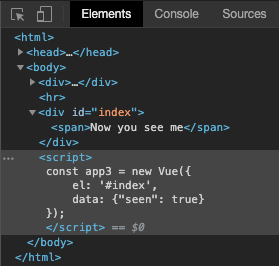
\includegraphics[width=6cm]{Rysunki/Rozdzial4/VueFlaskKod.png}
		\caption{Kod źródłowy strony wygenerowanej na podstawie listingu \ref{code:VueFlaskKod}. Przeglądarka \textit{Safari 13.1} pod systemy \textit{MacOS}.}	
		\label{fig:kodFlaskVue}
	\end{figure}
	

Jeżeli spojrzeć~w kod źródłowy strony~w przeglądarce wówczas można zauważyć, jak wyglądają już wygenerowane dane~z serwera dla podanego przykładu~i zauważyć, że metoda \textit{tojson} zwraca dane przesłane~w formie akceptowanej jako obiekt języka \textit{Javascript}, idealnie wpasowując się~w strukturę danych wymaganych przez pole \textit{data} obiektu instancji \textit{Vue}. Co sprawie, że można nimi operować bezpośrednio~w kodzie \textit{HTMLa} poprzez odpowiednie dyrektywy\cite{vuejs} (w tym przypadku dyrektywę \textit{v-if}) biblioteki \textit{Vue.js}.



W prosty sposób osiągnięto komunikację między serwerem, a biblioteką odpowiadającą za warstwę prezentacji. Niepotrzebne byłoby żadne dodatkowe narzędzie wystarczyło tylko wykorzystać elementy dostępne~w ramach obu tych frameworków.

Istnieją biblioteki pozwalające na szybkie tworzenie komponentów~w \textit{Vue}, nazywane \textit{UI Component Frameworks}. Są to zbiory gotowych elementów, do których wystarczy przekazać odpowiednio sformatowane dane~i ustawienia, a wygenerują one żądany fragment interfejsu użytkownika. W razie, gdy dostarczony komponent nie wygląda odpowiednio lub ma za mało funkcji to takie frameworki dostarczają proste \textit{API} do edycji ich wyglądu lub zastosowania, ale~w większości przypadków ich ustawienia~i dostępne możliwości są na tyle bogate, że ich większe zmiany są sporadyczne. Zastosowaną biblioteką~w projekcie jest \textit{ElementUI}\footnote{Link do dokumentacji \textit{ElementUI}: \url{https://element.eleme.io/}.}, można ją pobrać~z strony dokumentacji lub serwisu \textit{Github}\footnote{Link do repozytorium \textit{ElementUI} w serwisie \textit{github}: \url{https://github.com/ElemeFE/element}.} następnie przenieść do folderu \verb|static/js| i odpowiednio dodać do referencję~w pliku \textit{base.html} do:
 \begin{itemize}
  \item skryptu języka \textit{Javascript}: \verb|js/element-2.13.2/lib/index.js|
  \item arkuszy stylów biblioteki: \verb|js/element-2.13.2/lib/theme-chalk/index.css|
\end{itemize}

W folderze \textit{static/css} znajduje się plik \textit{main.css} odpowiada on za wszystkie style napisane~w projekcie monolitycznym~i podobnie do bibliotek~w języku \textit{Javascript} został on dołączony do pliku \textit{base.html}, więcej~o kaskadowych arkuszach stylów można przeczytać~w dokumentacji fundacji \textit{Mozilla}\cite{mdn}.
